\documentclass{standalone}

\RequirePackage{times}
\RequirePackage{amsmath}
\RequirePackage{amssymb}
\RequirePackage[T1]{fontenc}

\usepackage{tikz}
\usepackage{xcolor}
\usepackage{pgfplots}

\begin{document}
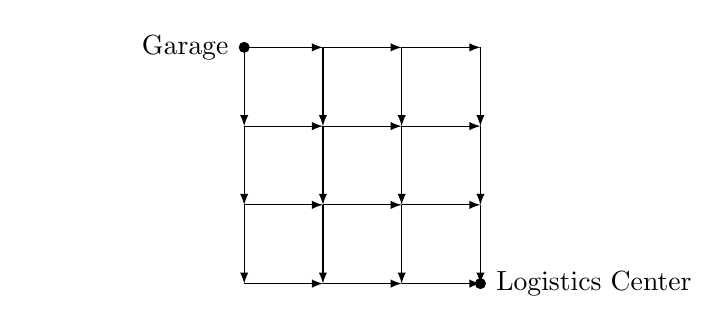
\begin{tikzpicture}
	\draw[-latex] (0,3) -- (1,3);
	\draw[-latex] (1,3) -- (2,3);
	\draw[-latex] (2,3) -- (3,3);
	\draw[-latex] (0,2) -- (1,2);
	\draw[-latex] (1,2) -- (2,2);
	\draw[-latex] (2,2) -- (3,2);
	\draw[-latex] (0,1) -- (1,1);
	\draw[-latex] (1,1) -- (2,1);
	\draw[-latex] (2,1) -- (3,1);
	\draw[-latex] (0,0) -- (1,0);
	\draw[-latex] (1,0) -- (2,0);
	\draw[-latex] (2,0) -- (3,0);
	\draw[-latex] (0,3) -- (0,2);
	\draw[-latex] (0,2) -- (0,1);
	\draw[-latex] (0,1) -- (0,0);
	\draw[-latex] (1,3) -- (1,2);
	\draw[-latex] (1,2) -- (1,1);
	\draw[-latex] (1,1) -- (1,0);
	\draw[-latex] (2,3) -- (2,2);
	\draw[-latex] (2,2) -- (2,1);
	\draw[-latex] (2,1) -- (2,0);
	\draw[-latex] (3,3) -- (3,2);
	\draw[-latex] (3,2) -- (3,1);
	\draw[-latex] (3,1) -- (3,0);
	
	\useasboundingbox (-2.75,-0.25) rectangle (5.75,3.25);
	
	\node[circle,fill=black,inner sep=0pt,minimum size=4pt,label=left:{Garage}] at (0,3) {};
	\node[circle,fill=black,inner sep=0pt,minimum size=4pt,label=right:{Logistics Center}] at (3,0) {};
\end{tikzpicture}
\end{document}